% SPDX-FileCopyrightText: 2023 SAP SE
%
% SPDX-License-Identifier: Apache-2.0
%
% This file is part of FEDEM - https://openfedem.org

%%%%%%%%%%%%%%%%%%%%%%%%%%%%%%%%%%%%%%%%%%%%%%%%%%%%%%%%%%%%%%%%%%%%%%%%%%%%%%%%
%
% FEDEM User Guide.
%
%%%%%%%%%%%%%%%%%%%%%%%%%%%%%%%%%%%%%%%%%%%%%%%%%%%%%%%%%%%%%%%%%%%%%%%%%%%%%%%%

\Chapter{Control System Modeling}{control-system-modeling}

Real mechanisms are often connected to or acted upon by control elements such as
sensors, controllers, and actuators. A control system is therefore necessary to
simulate these effects for Fedem mechanisms.
This chapter describes the control elements available in the Fedem Control
System library, and explains how to model your control systems.

Sections in this chapter address the following topics:

\begin{itemize}
\item
  \protect\hyperlink{control-modeling-environment}
                    {Control modeling environment}
\item
  \protect\hyperlink{input-and-output}
                    {Input and output}
\item
  \protect\hyperlink{control-blocks}
                    {Control blocks}
\item
  \protect\hyperlink{building-control-modules}
                    {Building control modules}
\end{itemize}

\clearpage


%%%%%%%%%%%%%%%%%%%%%%%%%%%%%%%%%%%%%%%%%%%%%%%%%%%%%%%%%%%%%%%%%%%%%%%%%%%%%%%%
\Section{Control modeling environment}{control-modeling-environment}

The block-diagram presentation of the control systems in Fedem closely resembles
what is given in most textbooks about basic control theory.
The graphical representation consists of a series of connected control blocks,
which you can model to simulate your control requirements.


\SubSection{Control Editor}{control-editor}

To create a control system, Fedem provides the {\sl Control Editor} view in
which control systems can be created and manipulated. Control blocks are
selected from the \textbf{Control} menu or the \textbf{Control Creation}
tool bar for placement in the {\sl Control Editor} view.
They can then be moved and manipulated with drag-and-drop functionality.
This editing environment also features grid and snap functionality
(see \refSection{setting-grid-and-snap}{Setting Grid and Snap}).

\vskip\parskip
\IconText{controlEditor}{
  To open the {\rm Control Editor}, click the \textbf{Show Control Editor}
  button on the \textbf{Windows} menu or tool bar.
  The {\sl Control Editor} view is shown below with an example control system.
}
\begin{figure}[!h]
  \center\vskip-2mm % Trim off some white space around this image
  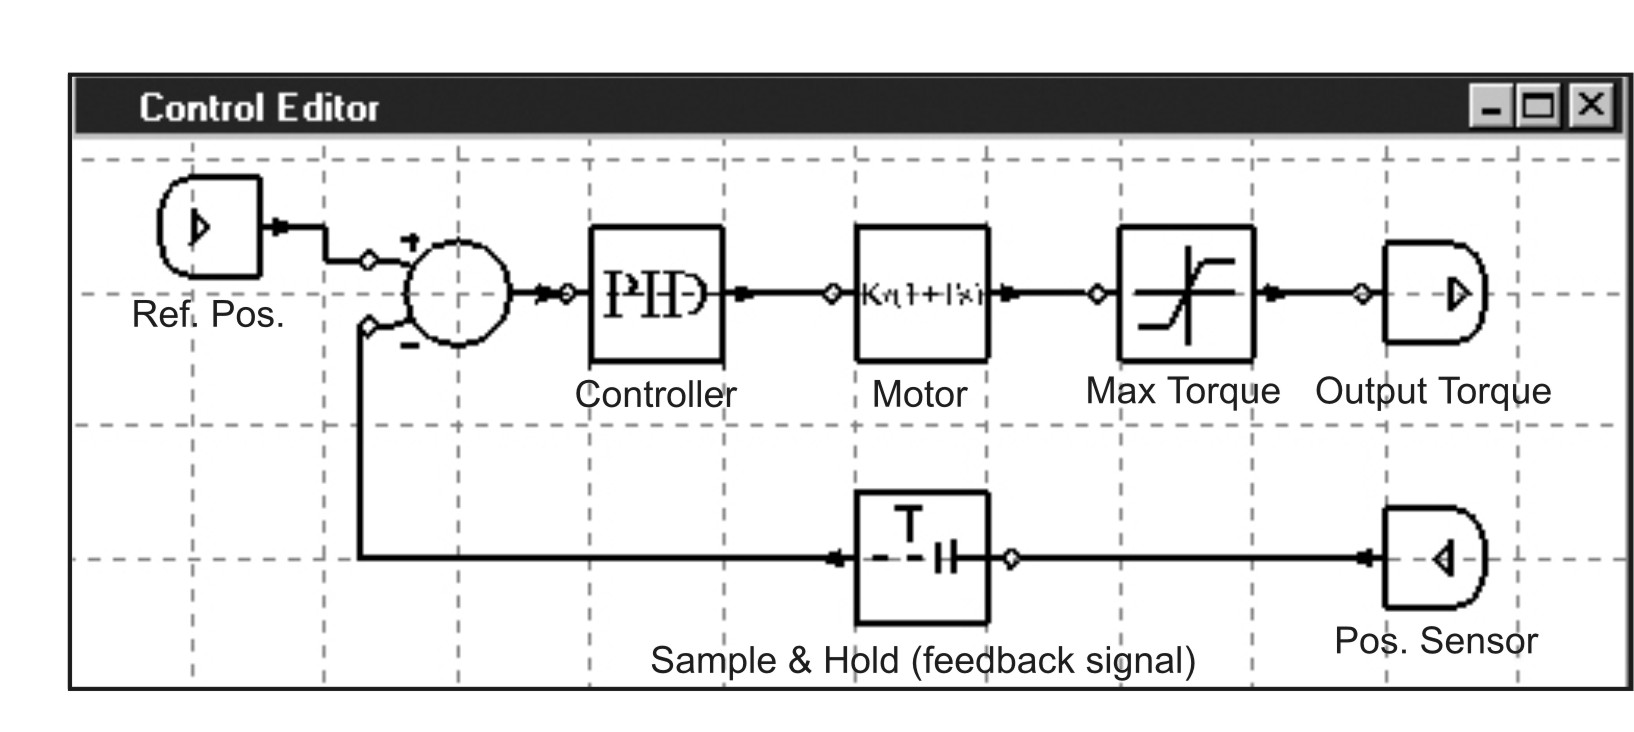
\includegraphics[trim=0 10 0 17,clip,width=0.85\textwidth]{Figures/cs ricardo}
\end{figure}


\SubSection{Control tool bars}{control-tool-bars}

Fedem provides two tool bars for modeling control systems:


\subsubsection{Control Creation tool bar}

The \textbf{Control Creation} tool bar (shown below) consists of the Fedem
control blocks that are used to build control modules.
(See \refSection{control-blocks}{Control blocks} for descriptions of each
control block).

\begin{figure}[!h]
  \center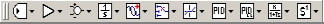
\includegraphics[width=0.85\textwidth]{Figures/Control Entities Toolbar}
\end{figure}


\subsubsection{Control Tools tool bar}

\begin{wrapfigure}{r}{0.25\textwidth}
  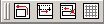
\includegraphics[width=0.25\textwidth]{Figures/Controls Toolbar}
\end{wrapfigure}

The \textbf{Control Tools} tool bar (shown to the right)
consists of drawing and editing tools.
(See \refSection{building-control-modules}{Building control modules}
for use of these commands.)


\SubSection{Control system topology}{control-system-topology}

\begin{wrapfigure}{r}{0.3\textwidth}
  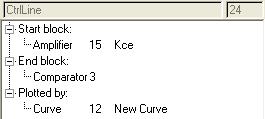
\includegraphics[width=0.3\textwidth]{Figures/5-Control-System-Topo}
\end{wrapfigure}

In a similar manner as for the structural mechanism, the topology of the current
control system may be browsed in the {\sl Topology} view in the lower left
corner of the Fedem main window.
(See also \refSection{id-and-topology-panel}{ID and Topology panel}).


%%%%%%%%%%%%%%%%%%%%%%%%%%%%%%%%%%%%%%%%%%%%%%%%%%%%%%%%%%%%%%%%%%%%%%%%%%%%%%%%
\Section{Input and output}{input-and-output}

The input and output blocks are the connections through which the
control system and the rest of the mechanism model interact.

\subsubsection{Control Input}

\IconTextFirst{input}{
  The input block is used to set up input values from the mechanism,
  either measurements, or functions of time. The options of the Control Input
  element is nearly identical to the options of a Function.
  See \refSection{function-properties}{Function properties}. The output value
  of the Control Input is then connected to other control elements.}

\subsubsection{Control Output}

\IconTextFirst{output}{
  The output block is used to make a response variable from the control system
  available to the mechanism. When created, it will automatically be available
  in the various drop-down menus that allow values from a control system.
  The variable can then be used to control the magnitude of loads,
  changes in spring length, and so on.}

The Control output has the option to use an embedded function to alter the
output from the control system before it is applied to the mechanism.
This function is edited in the same way as Functions.
See \refSection{function-properties}{Function properties}.


%%%%%%%%%%%%%%%%%%%%%%%%%%%%%%%%%%%%%%%%%%%%%%%%%%%%%%%%%%%%%%%%%%%%%%%%%%%%%%%%
\Section{Control blocks}{control-blocks}

The {\sl Control blocks} (also called control elements) calculate the output as
a function of one or more inputs and the block's internal state.
When a control element is selected in the {\sl Control Editor} view,
its mathematical equation and properties are shown in the Property Editor panel
(see \refSection{editing-block-properties}{Editing block properties}).
For more information about individual control elements,
see the \FedemTGuide{Chapter 8, "Control System"}.

The following sections describe the control elements available for use in
Fedem control systems.


\SubSection{Amplifiers}{amplifiers}

The control system supports the two types of amplifiers described below:

\bigskip\IconText{amplifier}{
  \textbf{Amplifier block} \\[1mm]
  The Amplifier block amplifies the input signal with a user-defined value.}

\bigskip\IconText{power_block}{
  \textbf{Power block} \\[1mm]
  The power block calculates and outputs the power ($n$) of the input signal
  ($x$), where $n$ is specified by the user.}


\SubSection{Binary-input blocks}{binary-input-blocks}

Binary-input control elements have two input signals.
The binary input blocks used in Fedem have no editable parameters.
Each block is described below.
(See also the \FedemTGuide{Section 8.4.1, "Basic elements"}.)

\medskip\IconText{comparator}{
  \textbf{Comparator block} \\[1mm]
   The comparator block calculates and outputs the difference between the
   two input signals.}

\medskip\IconText{adder}{
  \textbf{Adder block} \\[1mm]
  The Adder block adds the two input signals and outputs the sum.}

\medskip\IconText{multiplier}{
  \textbf{Multiplier block} \\[1mm]
  The multiplier block multiplies tthe input signals and outputs the product.}


\SubSection{Integrator and limited derivator blocks}
           {integrator-and-limited-derivator-blocks}

Fedem supports the use of the integrator and limited derivator blocks
described below. (See also the \FedemTGuide{Section 8.4.1, "Basic elements"}.)

\medskip\IconText{integrator}{
  \textbf{Integrator block} \\[1mm]
  The Integrator block outputs the integral of the input signal.}

\medskip\IconText{derivator}{
  \textbf{Derivator block} \\[1mm]
  The Derivator block outputs the derivative of the input signal within
  a specified bandwidth.}


\SubSection{Time-dependent blocks}{time-dependent-blocks}

The control system supports two time-dependent control blocks described below.
(See also the \FedemTGuide{Section 8.4.2, "Time-dependent elements"}.)

\medskip\IconText{timeDelay}{
  \textbf{Delay block} \\[1mm]
  The Delay block outputs a delayed input signal.}

\medskip\IconText{sampleAndHold}{
  \textbf{Sample-and-Hold} \\[1mm]
  The Sample-and-Hold block outputs a sampled input signal.}


\SubSection{Non-continuous blocks}{non-continuous-blocks}

Non-continuous control blocks are used for simulating nonlinear behavior.
They are used when the system response cannot be described by a linear model.
(See also the \FedemTGuide{Section 8.4.3, "Piecewise continuous elements"}.)

\medskip\IconText{logicSwitch}{
  \textbf{Logical-Switch block} \\[1mm]
  The Logical-Switch block returns one of two predefined constant inputs,
  both of which are dependent upon the value of a third input, called the
  control input. If the signal of the control input is greater than or equal to
  the threshold parameter, the block returns the user-specified upper limit;
  otherwise, it returns the user-specified lower limit.}

\medskip\IconText{limitation}{
  \textbf{Limiter block} \\[1mm]
  The Limiter block imposes upper and lower bounds on a signal.
  When the input signal is within the user-specified range of the upper and
  lower parameters, the input signal passes through unchanged.
  When the input signal is outside these limits,
  the signal is limited to the upper or lower limit.}

\medskip\IconText{deadZone}{
  \textbf{Dead-Zone block} \\[1mm]
  The Dead-Zone block generates zero output within a
  specified range called its {\sl dead zone}.
  The lower and upper limits of the dead zone are specified as the {\sl Left}
  and {\sl Right} parameters in the Property Editor panel.
  The block output depends on the input and the dead zone as follows:
  \begin{itemize}
  \item
    If the input is within the dead zone (greater than the lower limit and
    less than the upper limit), the output is zero.
  \item
    If the input is greater than or equal to the upper limit,
    the output is the input minus the upper limit.
  \item
    If the input is less than or equal to the lower limit,
    the output is the input minus the lower limit.
\end{itemize}}

\medskip\IconText{hysteresis}{
  \textbf{Hysteresis block} \\[1mm]
  The Hysteresis (backlash) block controls output in such a way that
  a change in input causes an equal change in the output. However,
  changes in direction of the input signal have no effect on the output. The
  amount of side-to-side play in the system is referred to as {\sl deadband}.
  The deadband is centered about the output.}


\SubSection{PI, PD, and PID controllers}{pi-pd-and-pid-controllers}

PI, PD, and PID controllers are used to control output in such a way that
the given input source forces a desired result.
PI, PD, and PID controllers are described in detail in the
\FedemTGuide{Section 8.4.4, "Compensator elements"}.
The following are controllers used in Fedem:

\medskip\IconText{PID}{\vspace{8pt}
  \textbf{PID Controller block}}

\medskip\IconText{PIC}{\vspace{8pt}
  \textbf{PI Controller block}}

\medskip\IconText{PD}{\vspace{8pt}
  \textbf{PD Controller block}}

\medskip\IconText{PlimI}{\vspace{8pt}
  \textbf{P Limited I Block (limited PI controller)}}

\medskip\IconText{PlimD}{\vspace{8pt}
  \textbf{P Limited D Block (limited PD controller)}}

\medskip\IconText{PIlimD}{\vspace{8pt}
  \textbf{PI Limited D Block (limited PID controller in serial form)}}

\medskip\IconText{PlimIlimD}{\vspace{8pt}
  \textbf{P Limited I and D Block (limited controller in serial form)}}


\SubSection{General-transfer functions}{general-transfer-functions}

General transfer functions are continuous mathematical functions used to
describe differential equations. The time response of the system is
characterized by poles (the roots of the functions).
Fedem uses the general transfer functions listed below.
For a detailed description, see the \FedemTGuide{Section 8.4.5,
"General transfer functions".}

\medskip\IconText{realPole}{
  \textbf{Real-Pole} \\[1mm]
  The Real-Pole block is a first-order transfer function.
  The Real-Pole block has a pole positioned on the real,
  negative axis in the $s$-plane.}

\medskip\IconText{complex-conj-pole}{
  \textbf{Complex Conjugate Pole block} \\[1mm]
  The Complex Conjugate Pole block is described by a second-order
  differential equation.}

\medskip\IconText{1stOrderTransferFunction}{
  \textbf{First-Order Transfer Function block} \\[1mm]
  The First-Order Transfer Function block is described in detail
  in the \FedemTGuide{Section 8.4.5} (see {\sl"First-order element"}).}

\medskip\IconText{2ndOrderTransferFunction}{
  \textbf{Second-Order Transfer Function block} \\[1mm]
  The Second-Order Transfer Function block is described in detail
  in the \FedemTGuide{Section 8.4.5} (see {\sl"Second-order element"}).}


%%%%%%%%%%%%%%%%%%%%%%%%%%%%%%%%%%%%%%%%%%%%%%%%%%%%%%%%%%%%%%%%%%%%%%%%%%%%%%%%
\Section{Building control modules}{building-control-modules}

The control module is fully defined when all blocks are connected and the inputs
and outputs are attached to sensors and actuators in the mechanism model.


\SubSection{Setting Grid and Snap}{setting-grid-and-snap}

\IconTextFigure{controlEditorGrid}{
  You can manipulate the Grid and Snap settings in the
  {\sl Control Editor} view by selecting the \textbf{Control Editor Grid/Snap}
  button from the \textbf{Tools} menu or the \textbf{Control Tools} tool bar.
  The Grid and Snap dialog box is then opened (shown at right).
  %
  \noindent
  %Can't use the \Note macro here since we are inside a tabular environment
  \begin{picture}(200,40)
    \put(-50,10) {
\includegraphics[width=8mm]{Figures/note}}
    \put(-4,15) {
      \begin{minipage}{0.63\textwidth}
        \sl\textbf{NOTE}:
        Grid and Snap options are applicable only for the Control Editor view.
      \end{minipage}}
  \end{picture}
}{Figures/5-grid-and-snap}

\SubSection{Inserting blocks}{inserting-blocks}

To insert control system blocks, complete the following steps:

\begin{enumerate}
\item
  Click the button that represents the block you want to insert.

  \EnumTip{
    You may have to hold down the arrow found next to a block of a similar
    type to access the drop-down menu with other block selections.}

\item
  Move the cursor into the {\sl Control Editor} view.
  You will see the block following the mouse.
  Place the block where you want it and click the left mouse button to drop it.
\end{enumerate}

\Note{When a block is inserted in the Control Editor view,
  it is automatically added to the Model Manager Objects list.}


\SubSection{Moving blocks}{moving-blocks}

You can adjust the block position by positioning the cursor over the block,
pressing the left mouse button, and dragging the block to the new position.
When the block is correctly positioned, release the mouse button.

Several blocks can also be moved together. To do that, press and hold
the \textbf{Ctrl} key, then select the blocks you want to move and finally
drag them to the new position.


\SubSection{Editing block properties}{editing-block-properties}

Once a block is inserted in the {\sl Control Editor} view,
you can select it and editing its properties in the Property Editor panel.
For example, the equation and properties of a PID control block are shown below.

\begin{figure}[!h]
  \center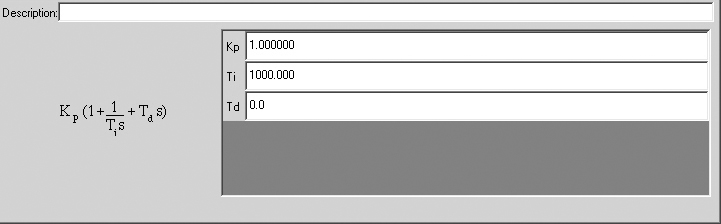
\includegraphics[width=0.8\textwidth]{Figures/PID properties}
\end{figure}

\Caution{Changing a value in the Property Editor panel does not automatically
  apply the change. You must press the \textbf{Enter} key after editing each
  value to apply the change.}


\SubSection{Connecting blocks}{connecting-blocks}

\noindent
\begin{minipage}{0.55\textwidth}
  \raggedright
  Once you have placed blocks in the {\sl Control Editor} view, you must draw
  connection lines between them to define the control module (shown at right).
  To connect two control blocks in your control module, do the following steps:

  \vskip1mm
  \begin{bulletlist}
    \setlength\itemsep{1mm}
  \item Click and drag from the arrow (output) of one control block ---
  \item ---to the circle (input) of another block and release the mouse button.
  \end{bulletlist}
\end{minipage}% <--- the % is needed here to kill off spurious spacing
\hfill\begin{minipage}{0.4\textwidth}
  \begin{picture}(140,80)
    \put(0,0){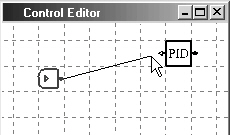
\includegraphics[width=\textwidth]{Figures/5-Connecting-Block}}
    \put(35,20){\Bullet{1}}
    \put(81,50){\Bullet{2}}
  \end{picture}
\end{minipage}

\vskip\parskip
A connection line is then drawn between the two blocks.
You can adjust the path of the line by dragging and dropping the line.
Click and drag either a corner or a line segment between the corners.


\subsubsection{Adding break points}

\IconTextFirst{addBreakpoint}{
  This command adds lines or breaking points to connection lines. To use it,
  click the \textbf{Add Breakpoint} button on the \textbf{Control Tools}
  tool bar, then click and drag an existing line. A new corner is created.}

\subsubsection{Removing break points}

\IconTextFirst{removeBreakpoint}{
  This command removes lines or breaking points on connection lines. To use it,
  click the \textbf{Remove Breakpoint} button on the \textbf{Control Tools}
  tool bar, then select one of the break points on a line.
  Press \textbf{Done} to confirm the selection.}

\Note{A line consists of at least three perpendicular line segments.
  It is not possible to remove line points/segments if doing so reduces
  the line to less than three segments.}

\Note{Changing the path or breakpoints of a line is for display purposes only
  and has no influence on control system performance.}


\SubSection{Rotating blocks}{rotating-blocks}

\IconTextFirst{flipElement}{
  You can rotate control blocks $180^\circ$, so that the input connections are on
  the right side of the block, and the output connections are on the left side.
  To rotate a block, click the \textbf{Flip Element Direction} button
  on the \textbf{Control Tools} tool bar and select the block.
  Press \textbf{Done} to confirm the selection.}

\Note{This command is for display purposes only and has no influence on control
  system performance.}


\SubSection{Deleting blocks or connections}{deleting-blocks-or-connections}

To delete a block or connection line in the {\sl Control Editor} view,
complete the following steps:

\begin{enumerate}
\item
  Select the line or block in the {\sl Control Editor} view.

  \EnumNote{You can select multiple blocks at the same time by selecting them
    in the Model Manager {\rm Objects} list.}

\item
  Click the \textbf{Delete} button on the \textbf{Standard} tool bar,
  or the \textbf{Delete} key on the keyboard.
  The selected objects are removed from the control system.
\end{enumerate}

\vskip-14mm
\IconText{delete}{\vspace*{8mm}\mbox{}}

\Note{When you delete a block,
  all connection lines to and from the block are also removed.}
